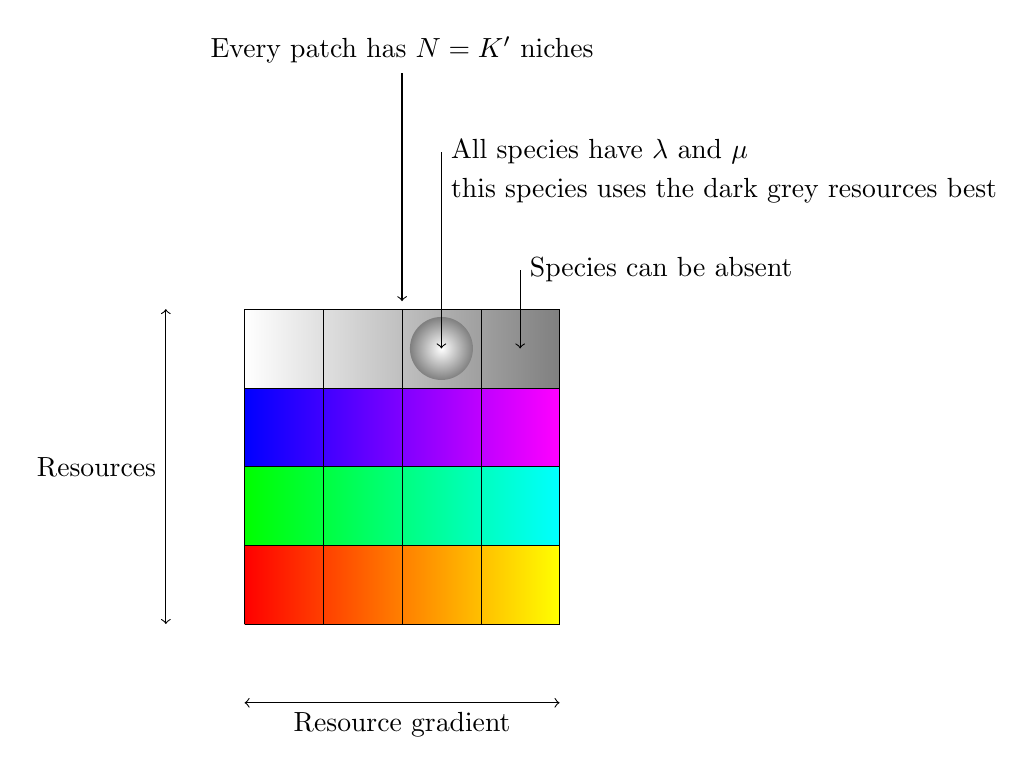
\begin{tikzpicture} 
  % Patch gradients
  \shade[left color=red,right color=yellow] (0,0) rectangle (4,1);
  \shade[left color=green,right color=cyan] (0,1) rectangle (4,2);
  \shade[left color=blue,right color=magenta] (0,2) rectangle (4,3);
  \shade[left color=white,right color=gray] (0,3) rectangle (4,4);
  % Species gradients
  \shade[inner color=white,outer color=gray] (2.5,3.5) circle (0.4 cm);
  % Grids
  \draw[step=1cm,black,very thin] (0,0) grid ( 4,4); 
  %\draw[step=1cm,gray,very thin] (6,0) grid (10,4); 
  % Arrows
  %\draw[<->,gray] (4+0.1,2) -- (5,2) node[anchor=south] {$m$} -- (6-0.1,2);
  \draw[<->] (0,-1) -- (2,-1) node[anchor=north] {Resource gradient} -- (4,-1) ;
  \draw[<->] (-1,0) -- (-1,2) node[anchor=east] {Resources} -- (-1,4) ;
  \draw[<-] (2,4+0.1) -- (2.0,7) node[anchor=south] {Every patch has $N = K'$ niches};
  \draw[<-] (2.5,3.5) 
    -- (2.5,5.5) node[anchor=west] {this species uses the dark grey resources best}
    -- (2.5,6) node[anchor=west] {All species have $\lambda$ and $\mu$};
  \draw[<-] (3.5,3.5) -- (3.5,4.5) node[anchor=west] {Species can be absent};
\end{tikzpicture}